%To check the light-tightness of the dark box, the PMT dark current was measured before and after covering the setup by a special black blanket from Thorlabs \cite{BlackBlancket}, that prevents external photons from entering the system. No statistically significant differences was observed between the covered and uncovered setup, which indicates that the black box is sufficiently light tight. 
The experimental setup was placed in a light-tight box. The light-tightness of the box was carefully test. The optimal PMT HV was selected from the plot of the photocurrent as a function of the first dynode voltage as the voltage at the beginning of the plateau. At this HV the $CE$ is equal to 1 and no secondary electrons are produced. This plot was measured between $0$ and $800~\volt$ without fibers, first with the LED off (PMT dark current) and then with the LED current at $1~\milli\ampere$. The number of photons detected by the PMT (difference between both spectra) is plotted in Figure \ref{fig:PlateauNoGainPMT}. As it can be seen, the plateau starts at voltages higher than $150~\volt$. The selected voltage for the characterization was $250~\volt$.

\begin{figure}[h]
\centering
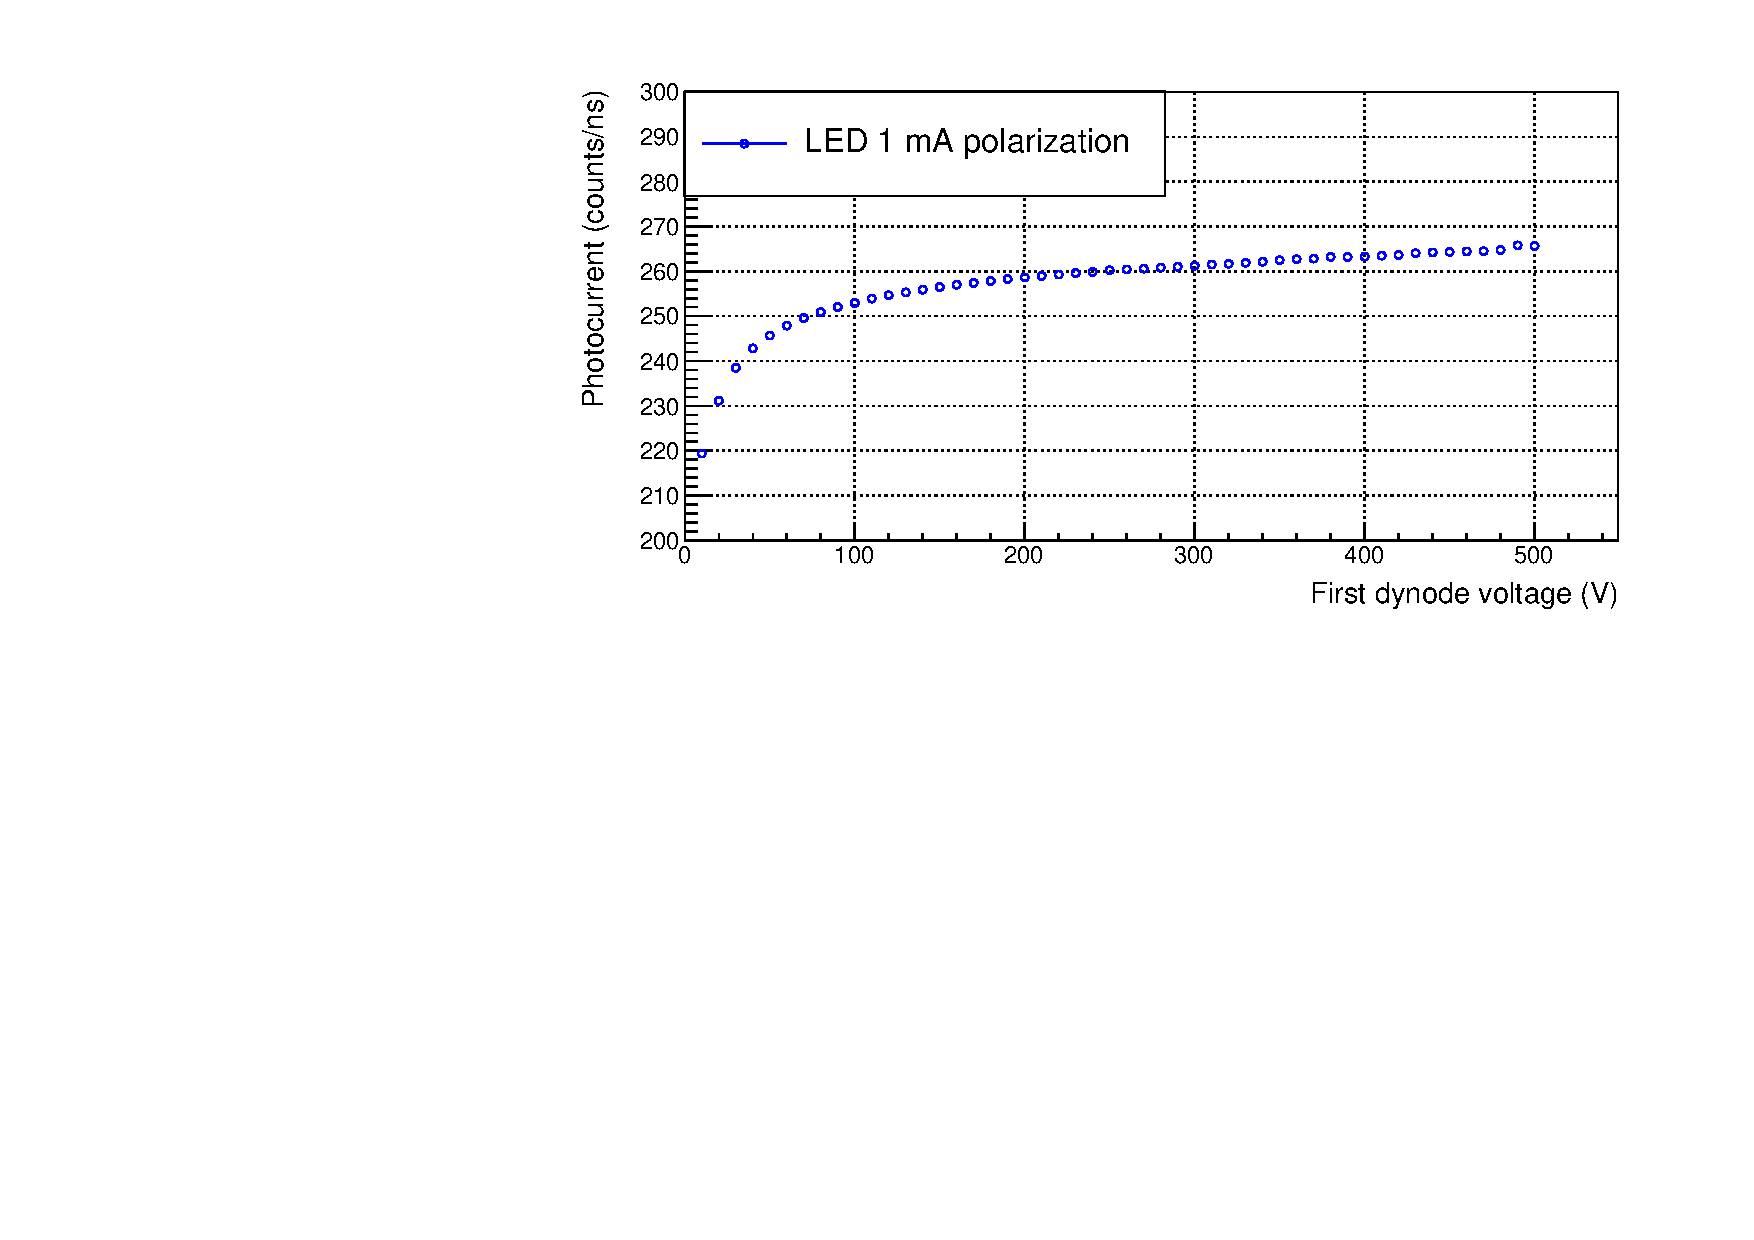
\includegraphics[scale=0.7]{4ResearchAndDevelopments/41Fibers/PCBNoGainPlateau_Calibrated.pdf}
\caption{PMT photocurrent as a function of the first dynode voltage. Error bars are smaller than dot size.\label{fig:PlateauNoGainPMT}}
\end{figure}

The linear response of the PMT was verified in two different ranges, $~\text{photons}/\nano\second$, which is the expected number of photons for tritium events, and up to $\sim 2500~\text{photons}/\nano\second$, which is the range used for the fiber characterization. The linearity test of the PMT was performed in abscence of fibers. The results in the low and high illumination cases are plotted in Figure \ref{fig:LinearityRangesOfPMT}, in which no saturation of the PMT response is observed.

\begin{figure}
\centering
    \begin{subfigure}[b]{1\textwidth}
    \centering
    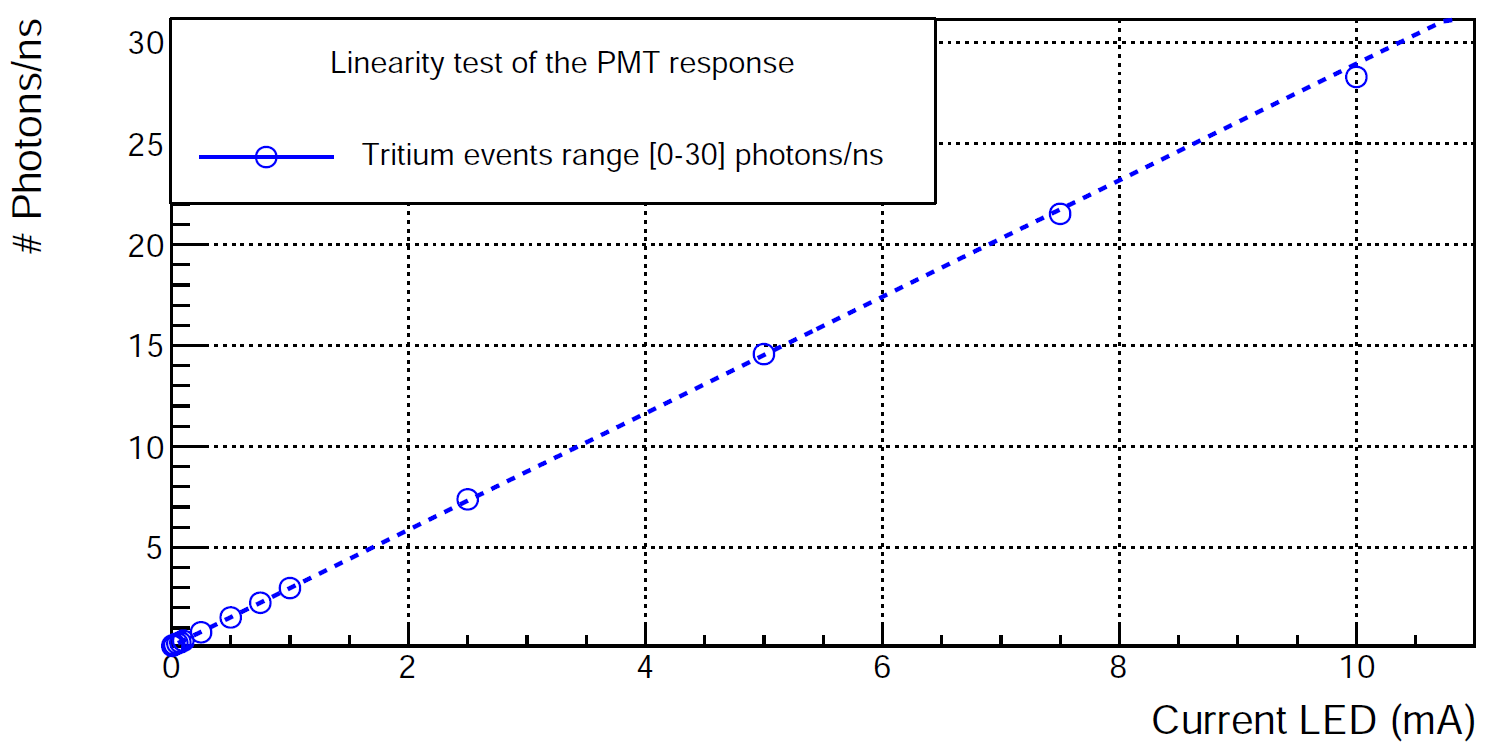
\includegraphics[scale=0.4,width=\textwidth]{4ResearchAndDevelopments/41Fibers/Linearity_test_0_30_range.png}  
    \caption{\label{subfig:LinearityTritiumRange}}
    \end{subfigure}
    \hfill
    \begin{subfigure}[b]{1\textwidth}
    \centering
    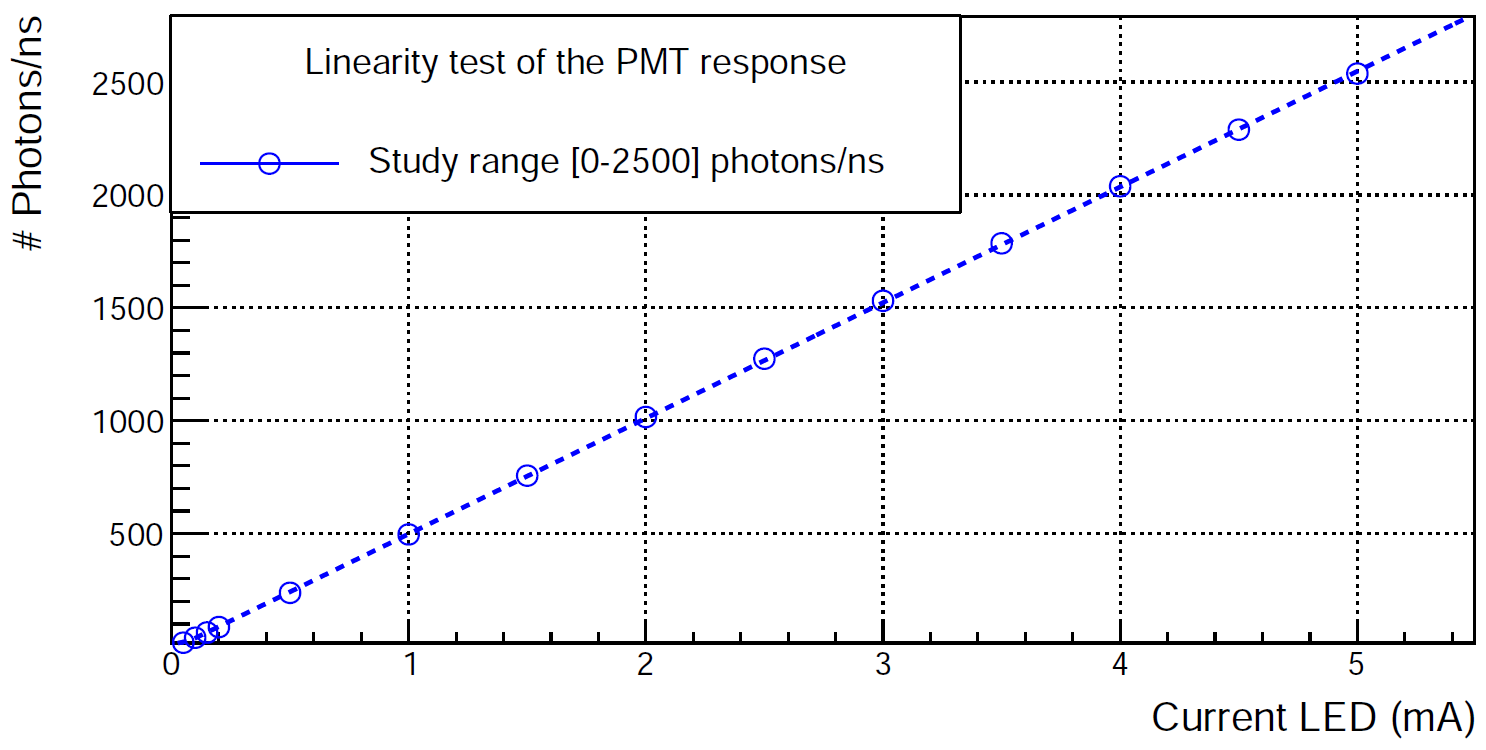
\includegraphics[scale=0.4, width=\textwidth]{4ResearchAndDevelopments/41Fibers/Linearity_test_0_2500_range.png}  
    \caption{\label{subfig:LinearityStudyRange}}
    \end{subfigure}
 \caption{Rate of photons measured by the PMT as a function of the LED current. a) Response of the PMT in the intensity range of tritium events. b) Response of the PMT in the range $0-2500~\text{photons}/\nano\second$. Error bars are smaller than the dot size.}
 \label{fig:LinearityRangesOfPMT}
\end{figure}